\section{Video Surveillance}\label{sec:video_surveillance}
Video surveillance is widely used to obtain documentation or evidence of a crime, or as a preventive tool.
As an example there is one camera for every 32 people in the United Kingdom\citep{london_camera_surveillance}.
This number includes both cameras installed by the government to surveil London, but also cameras installed by businesses to secure their property.
The high number of cameras is partially attributed to the high need for surveillance to prevent e.g. terrorist attacks in London, but additionally due to the technical difficulties of video surveillance. \\

A typical video surveillance solution consists of a set of cameras connected via cables to a ``command station''.
Video cameras are mounted on a fixed location, and can therefore only surveil an area limited by their field of view, see Figure~\ref{fig:camera_properties}, and the environment in which it is placed.\\

\begin{figure}[htb]
    \centering
    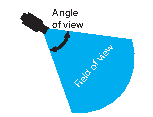
\includegraphics[scale=1.8]{gfx/camera_properties.pdf}
    \caption{A cameras field of view}
    \label{fig:camera_properties}
\end{figure}

An environment can contain physical objects which limits the cameras field of view further, see Figure~\ref{fig:refular_camera_setup}.
In small environments a sufficient surveillance-degree can be achieved without too much difficulty or cost\fixme{Statement - source til prisetr evt.}.
Properly surveilling large areas, in particular outdoor changing environments, is however problematic.\fixme{ref til Lytzen}

We have issues surveilling large areas, e.g. mink farms, with traditional solutions such as surveillance cameras.
The issues with a traditional solution for mink farms are that the establishment costs are very high due to e.g. digging.
% Vi har problemer med at overvåge store områder, som fx minkfarme, ved brug af en traditionel løsning i form af overvågningskameraer. Problemerne omkring en traditionel løsning til en minkfarm er at etableringsomkostninger er meget høje bl.a. på grund af gravearbejde.

%The need for video surveillance is based on the need for documentation of crimes, which is required in case of damage loses from an insurance perspective.
%Should a break-in occur a definitive proof of such must often be presented in order for insurances to cover potential losses.

Video cameras have a limited field of view, both in terms of vision and range, and only within this field of view is the quality high enough be usable as documentation.
This limitation can make it difficult and resource intensive to surveil large areas.
The resource intensitivity stems from the amount of hardware required to surveil, referring to both cameras, and the cables needed to connect the surveillance system.
The difficulty in surveilling the areas comes from the nature of an outdoor environment.
In terms of surveillance an indoor environment is static, as there is a limited amount of entrances and the interior of the buildings in terms of walls and doors remain the same.
In an outdoor environment the weather has to be taken into account.
The weather can be foggy, rainy, and the sun can blind a camera if it is improperly placed.
These conditions makes video surveillance of outdoor areas difficult.
Both indoors and outdoors does, however, have some challenges that needs to be faced, such as physical objects being moved around creating blind spots etc.

